\begin{frame}
\frametitle{About This Work...}

\emph{Finding Frequently Visited Indoor POIs Using Symbolic Indoor Tracking Data}.~\cite{lu2016finding} \\
H.~Lu, C.~Guo, B.~Yang, C.S.~Jensen.\\~\\

\begin{itemize}
  \item Published at \emph{EDBT' 2016}.
  \item Indoor flow counting methods on symbolic indoor tracking data are defined.
  \item Query related object uncertainty regions are derived by analysing the relationship between queries and tracking data.
  \item Make use of uncertainty analysis results to design algorithms for two specified query types.
\end{itemize}

\end{frame}

%------------------------------------------------

\begin{frame}
\frametitle{Motivation}

\begin{itemize}
  \setlength{\itemsep}{15pt}
  \item The indoor movements of people are increasingly datafied due to advances in indoor positioning.\cite{InLoc0:online}
    \begin{fitemize}
      \item indoor tracking data is being accumulated in a veriety of formats determined by the particular indoor positioning systems.
    \end{fitemize}

  \item Analyzing indoor tracking data can reveal how different parts of an indoor space are used.
    \begin{fitemize}
      \item the number of visits to a particular part of space over time.
    \end{fitemize}

  \item Flow counting in indoor spaces faces new, unique technical challenges.
  \begin{fitemize}
    \item uncertainties in indoor positioning systems
    \item indoor entities like doors and rooms enable as well as constrain the movement of indoor objects~\cite{DBLP:conf/edbt/YangLJ10}
  \end{fitemize}
\end{itemize}

\end{frame}

%------------------------------------------------

\begin{frame}
\frametitle{Notations}

\begin{figure}[tb]
  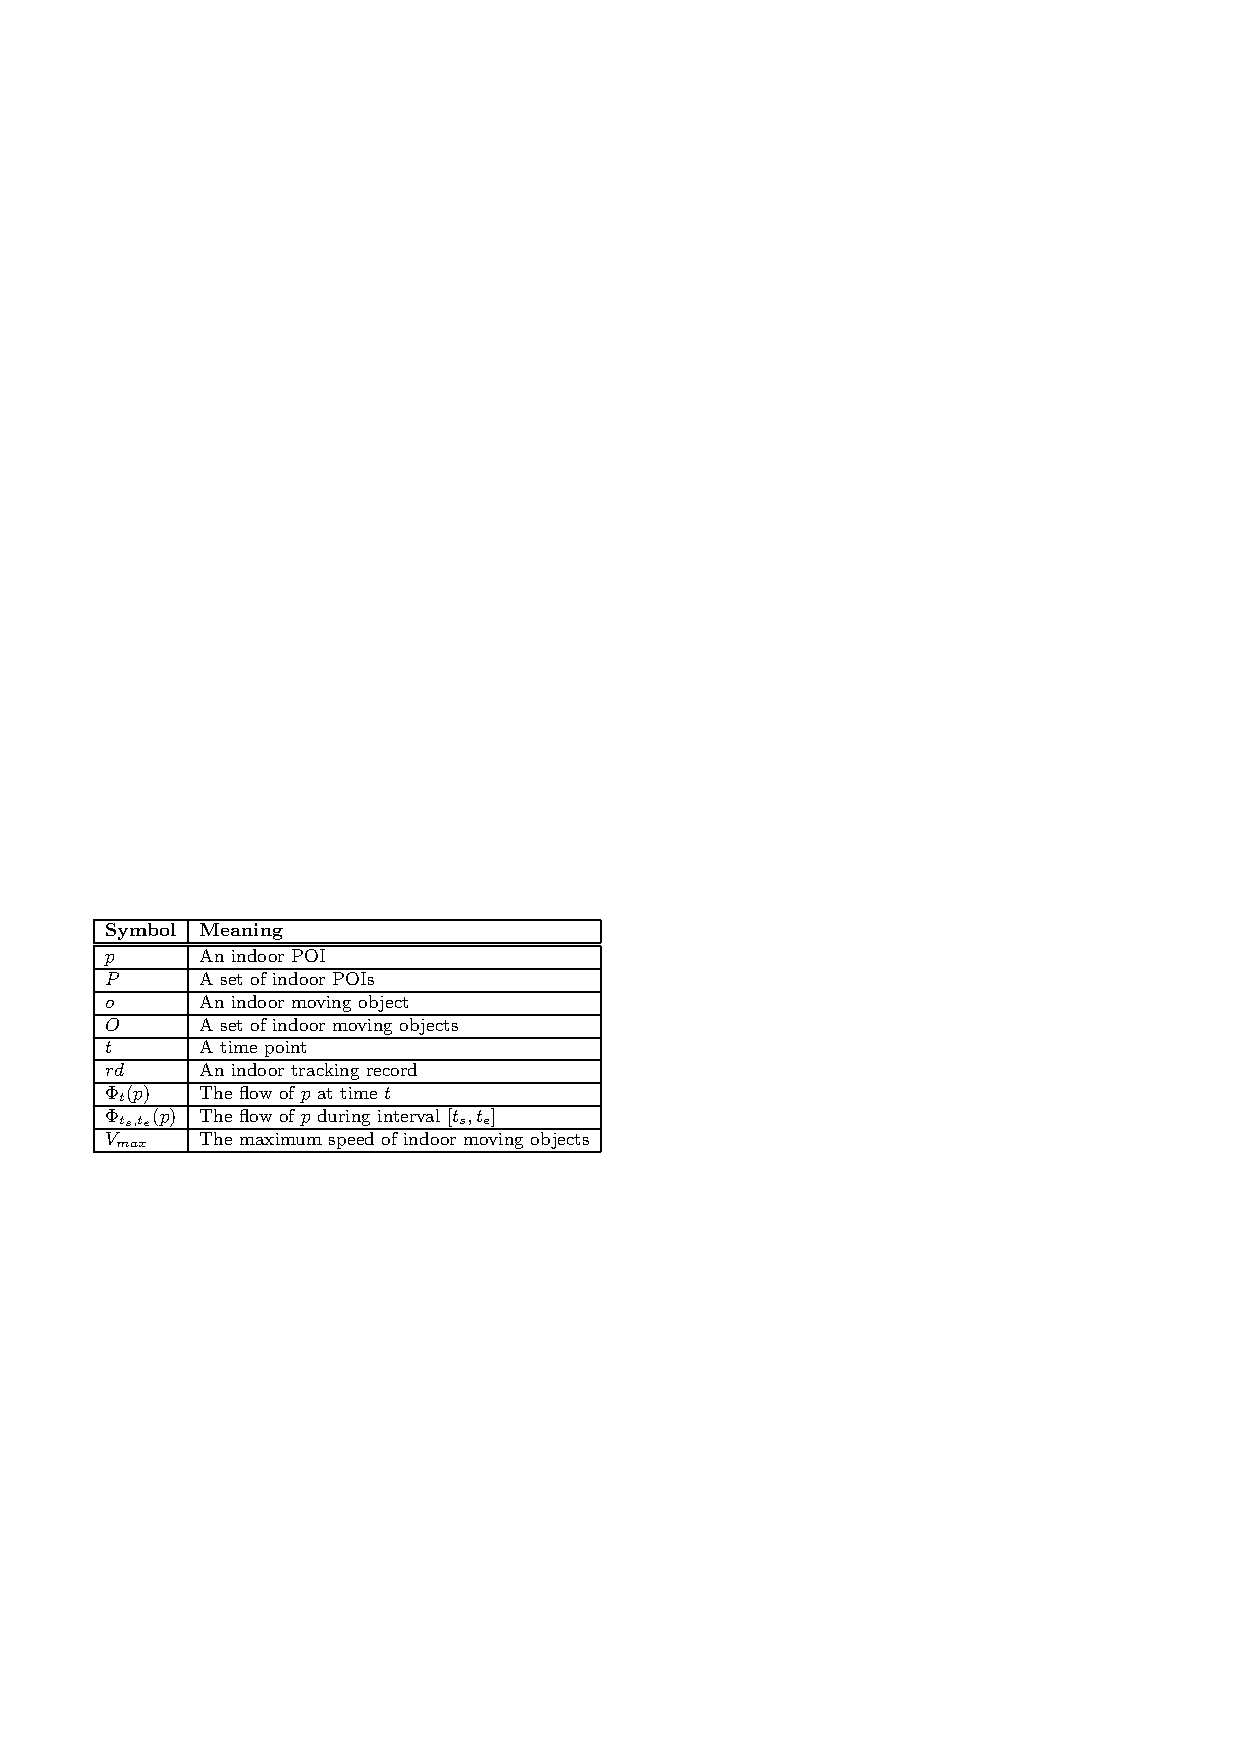
\includegraphics[width=0.94\columnwidth]{figures/4-1/4-1-1.pdf}
\end{figure}

\end{frame}

%------------------------------------------------

%------------------------------------------------

\begin{frame}
\frametitle{Preliminaries: Symbolic Indoor Tracking}

\begin{columns}[c]
  \column{.52\textwidth}
  \begin{figure}[tb]
    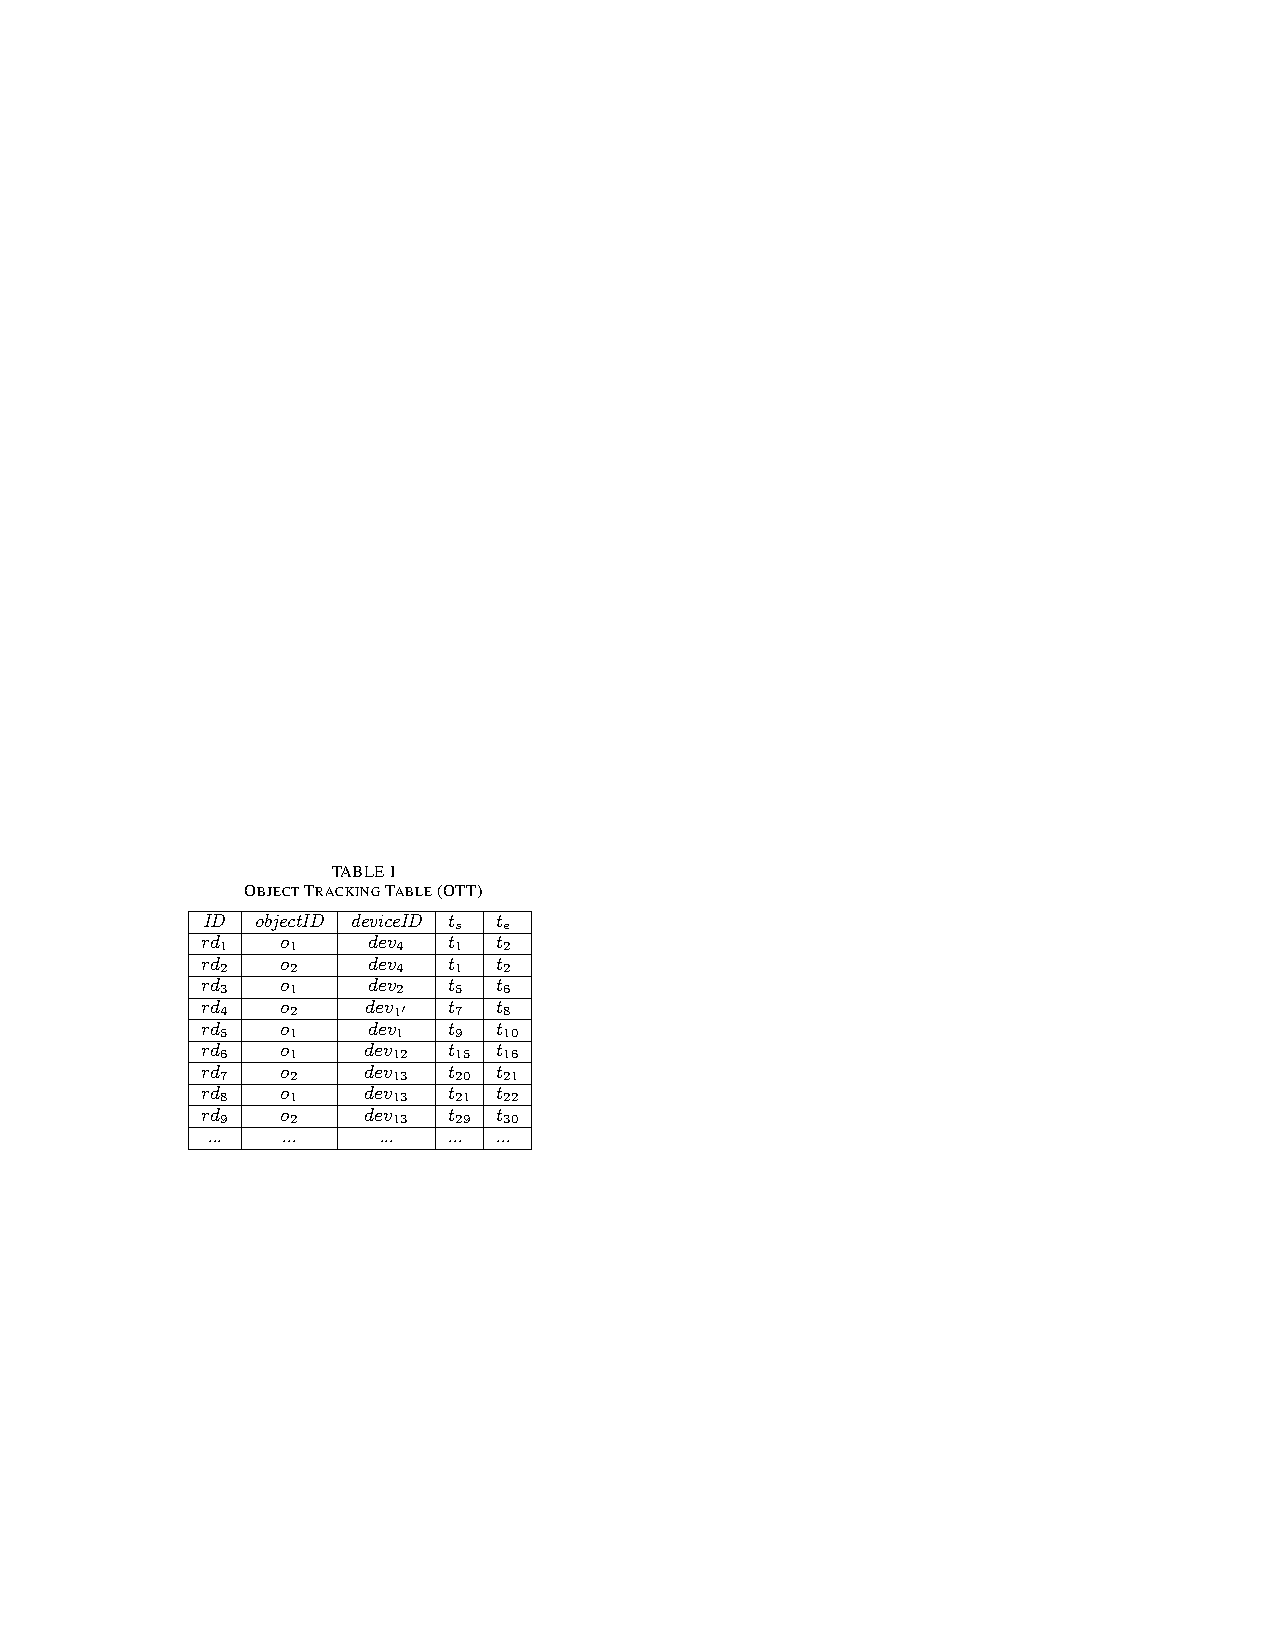
\includegraphics[width=\columnwidth]{figures/2-4/2-4-2.pdf}
  \end{figure}

  \column{.48\textwidth}
  \begin{fitemize}
    \item \conceptbf{Object Tracking Table} ${OTT}$ records the converted trajectories with schema ${(ID, objectID, deviceID, t_s, t_e)}$
    ~\\
    \item a record states that the object ${objectID}$ is observed by the device ${deviceID}$ in the closed interval from time ${t_s}$ to ${t_e}$.
  \end{fitemize}

\end{columns}

\end{frame}
